\section{Deep Reinforcement Learning}
\label{sec:rl}
In contrast to the manually developed algorithm, a Deep Q-learning based search algorithm was also developed. The agents is trained in using the simple simulator to search the map. Reinforcement learning suits this problem well as coverage can serve as a {\color{red} good} reward function. Traditional Q-learning methods store a table of discrete state-action pairs and their expected reward in memory {\color{red}[SOURCE]}. This table is called a Q-table. However, in real world applications state is often continuous, which creates the need to {\color{red} disoretize} the agent state. Another problem is that the size of the Q-table grows with the state space. Neural networks solve both of these problems. The Q-table can be approximated by using a neural network and then used to pick an action given a state.

Designing a neural network involves several important considerations. These include selecting the number of layers and neurons, choosing appropriate activation functions, and determining key hyperparameters such as the learning rate. After the architecture is defined, the network must be trained, evaluated, and iteratively optimized to ensure stable and effective learning. Finally, the trained model must be validated on unseen environments and integrated into the broader system for deployment.

\subsection{Network}
The general idea of a neural network is to construct a layered architecture where each layer, or tensor, consists of multiple interconnected neurons. Each neuron applies a learned weight and bias to its inputs and passes the result through an activation function. The final output of the network determines the action that the agent should take based on the current input state.

% TODO: How we use burn
This project utilize Burn \cite{burn}, which is a Rust Deep Learning Framework, for the implementation of the DQN. Burn provides a high-level API for building and training deep learning networks.

% TODO: Write how our network and activation function works (maybe in each of the models or only one?)
For this project, a feedforward fully connected neural network was used. The input to the network is a tensor representation part of the robot’s state, including sensor readings, and proximity to other robots. 
The output tensor represents descrete set of actions the robot can take. This is different values of steer angle and speed for the TurtleBot 4.
The network also consists of two hidden layers, with varying sizes depending on the model, and uses the ReLU (Rectified Linear Unit) activation function for all hidden layers.

\subsection{Reward}
The reward function is a central component of reinforcement learning, as it defines the learning signal by which the agent evaluates its actions. A well-designed reward function encourages desirable behavior and penalizes undesirable outcomes.

% TODO: Correct if we did not use negative reward
In this project, the reward is primarily based on map coverage. At each time step, a positive reward is given proportional to the amount of new area explored by the agent. This incentivizes the agent to move into unexplored regions of the map. Additionally, a small negative reward is applied for each step to encourage efficiency and to discourage the agent from idling or circling already explored areas.

% TODO: Correct if we did not use negative reward for range
To maintain network connectivity among robots, a penalty is also introduced if the agent moves outside of the communication range of the rest of the swarm. This helps reinforce coordinated exploration behavior, as isolated agents are less effective at contributing to the shared coverage objective. Collisions with obstacles are heavily penalized to promote safe navigation.

The final reward signal is a weighted sum of the above components and was empirically tuned to balance exploration, efficiency, and safety. This design guides the agent toward effective multi-robot collaboration while maintaining spatial awareness and mission goals.

\subsection{Training}
Training the neural network involves allowing the agent to interact with the environment over multiple episodes while incrementally improving its policy based on received rewards. A Deep Q-Network (DQN) approach is used, where the agent learns to approximate the optimal action-value function using a neural network.

Each training episode starts with the robot placed in a randomly generated environment, as described in the next subsection. The episode proceeds step by step, during which the agent observes its current state, selects an action using an $\epsilon$-greedy policy (balancing exploration and exploitation), executes the action, and receives a reward. The transition tuple $(s_t, a_t, r_t, s_{t+1})$ is stored in a replay buffer.

Mini-batches of transitions are sampled randomly from the replay buffer and used to train the network by minimizing the temporal-difference (TD) error. The target Q-value is computed using the Bellman equation:
$$Q_{\text{target}} = r_t + \gamma \max_{a'} Q(s_{t+1}, a')$$
where $\gamma$ is the discount factor.\\

Training continues for a fixed number of episodes or until the performance converges. An episode is terminated early if the agent fails to make significant progress (i.e., no new area is explored for a defined number of steps), or when the entire map is successfully covered.

The use of randomly generated maps with varying obstacle layouts (see Fig.~\ref{fig:generated-enviornments}) ensures that the agent generalizes its behavior across diverse spatial configurations, rather than overfitting to a single scenario.

\subsubsection{Generating Training Environments}
As to not overfit the network, it must be trained on many different environments. A simple program was created to generate worlds populated by line and circle obstacles.

\def\w{0.31\textwidth}
\begin{figure}[H]
    \begin{subfigure}{\w}
        \makebox(\textwidth, \textwidth)[\textwidth]{
            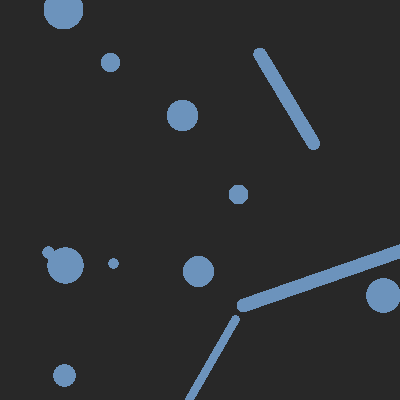
\includegraphics[width=\linewidth]{figures/generated-worlds/world_0.png}
        }
    \end{subfigure}
    \hspace*{\fill}
    \begin{subfigure}{\w}
        \makebox(\textwidth, \textwidth)[\textwidth]{
            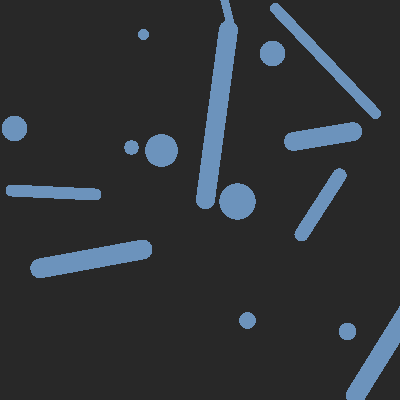
\includegraphics[width=\linewidth]{figures/generated-worlds/world_1.png}
        }
    \end{subfigure}
    \hspace*{\fill}
    \begin{subfigure}{\w}
        \makebox(\textwidth, \textwidth)[\textwidth]{
            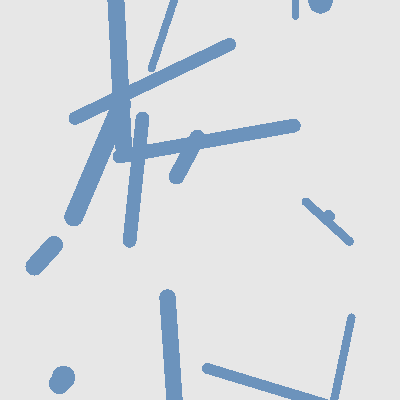
\includegraphics[width=\linewidth]{figures/generated-worlds/world_2.png}
        }
    \end{subfigure}

    \vspace{4mm}

    \begin{subfigure}{\w}
        \makebox(\textwidth, \textwidth)[\textwidth]{
            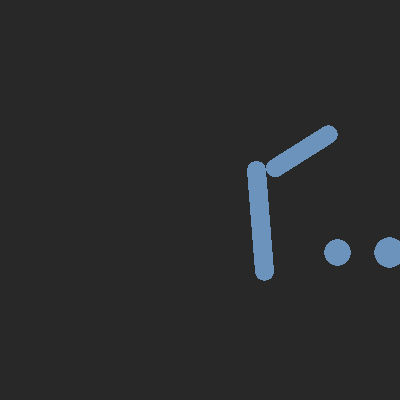
\includegraphics[width=\linewidth]{figures/generated-worlds/world_3.png}
        }
    \end{subfigure}
    \hspace*{\fill}
    \begin{subfigure}{\w}
        \makebox(\textwidth, \textwidth)[\textwidth]{
            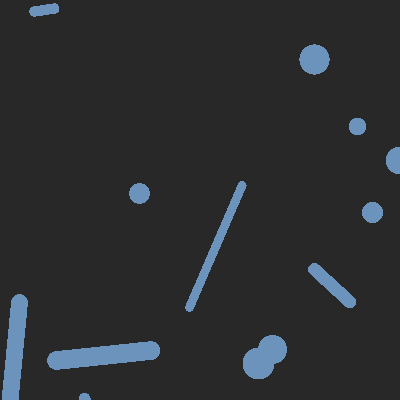
\includegraphics[width=\linewidth]{figures/generated-worlds/world_4.png}
        }
    \end{subfigure}
    \hspace*{\fill}
    \begin{subfigure}{\w}
        \makebox(\textwidth, \textwidth)[\textwidth]{
            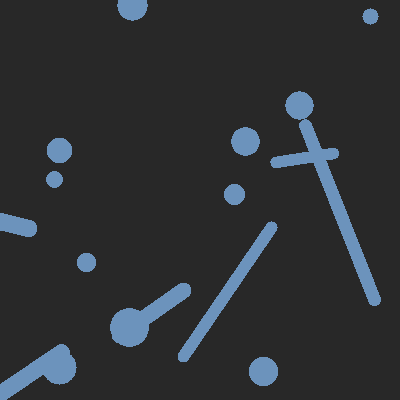
\includegraphics[width=\linewidth]{figures/generated-worlds/world_5.png}
        }
    \end{subfigure}
    \caption{Examples of generated environments} \label{fig:generated-enviornments}
\end{figure}
